\chapter{Déroulement du stage}

\begin{comment}
\paragraph{Préambule}
A mon arrivé à la centrale, j'ai été prié de regarder une vidéo de sécurité qui faisait le point  de tous les risques qu'on pouvait rencontrer et la façon de s'en protéger.

J'ai passé mon premier jour dans la lecture des documentations et j'ai eu l'occasion d'avoir une idée générale sur le fonctionnement de la centrale depuis la salle de contrôle. (Voir Annexe \uppercase\expandafter{\romannumeral 5}).

Une fois équipé du matériel de sécurité (voir annexe \uppercase\expandafter{\romannumeral 5}), je rejoint le terrain pour découvrir la centrale.

Dès la première semaine, j'ai participé à des sessions de maintenance en parallèle avec d'autres tâches (Conception d'une base de donnée).
\end{comment}
\section{Description du service maintenance}
Selon la définition de l'AFNOR, la maintenance vise à maintenir ou à rétablir un bien dans un état spécifié afin que celui-ci soit en mesure d'assurer un service déterminé.

La maintenance se décompose en 2 grandes familles : La maintenance préventive et la maintenance curative.

\textbf{La maintenance corrective : }La maintenance corrective (également appeler maintenance "pompier") consiste à laisser tourner une machine jusqu'à la casse afin d'effectuer les réparations nécessaires.

\textbf{La maintenance préventive : }La maintenance corrective entraînant des sur -coûts non négligeable, la maintenance préventive consiste à intervenir sur un équipement avant que celui-ci ne soit défaillant, afin de tenter de prévenir la panne. 

%\paragraph{Stratégie de la centrale}
Selon le contrat la liant avec la STEG, la CPC est payée non seulement pour sa production mais surtout pour sa disponibilité. C'est pourquoi au cours de mon stage j'ai effectué plus de travaux de maintenance préventive que corrective.
\section{Tâches effectuées au service maintenance}

\subsection{Analyse Thermographique}

\subsubsection{Principe et But}

La thermographie sert à mettre en évidence, par l'intermédiaire d'une caméra thermographique infrarouge, tout échauffement anormal lié au mauvais serrage, au mauvais sertissage de cosse, au sous-dimensionnement, à l'oxydation des contacts ou au déséquilibre de phase.

\subsubsection{Matériel de l'analyse}


Pour effectuer l'analyse thermographique on a principalement besoin d'une caméra thermographique infrarouge.
\begin{figure}[hbtp]
\centering
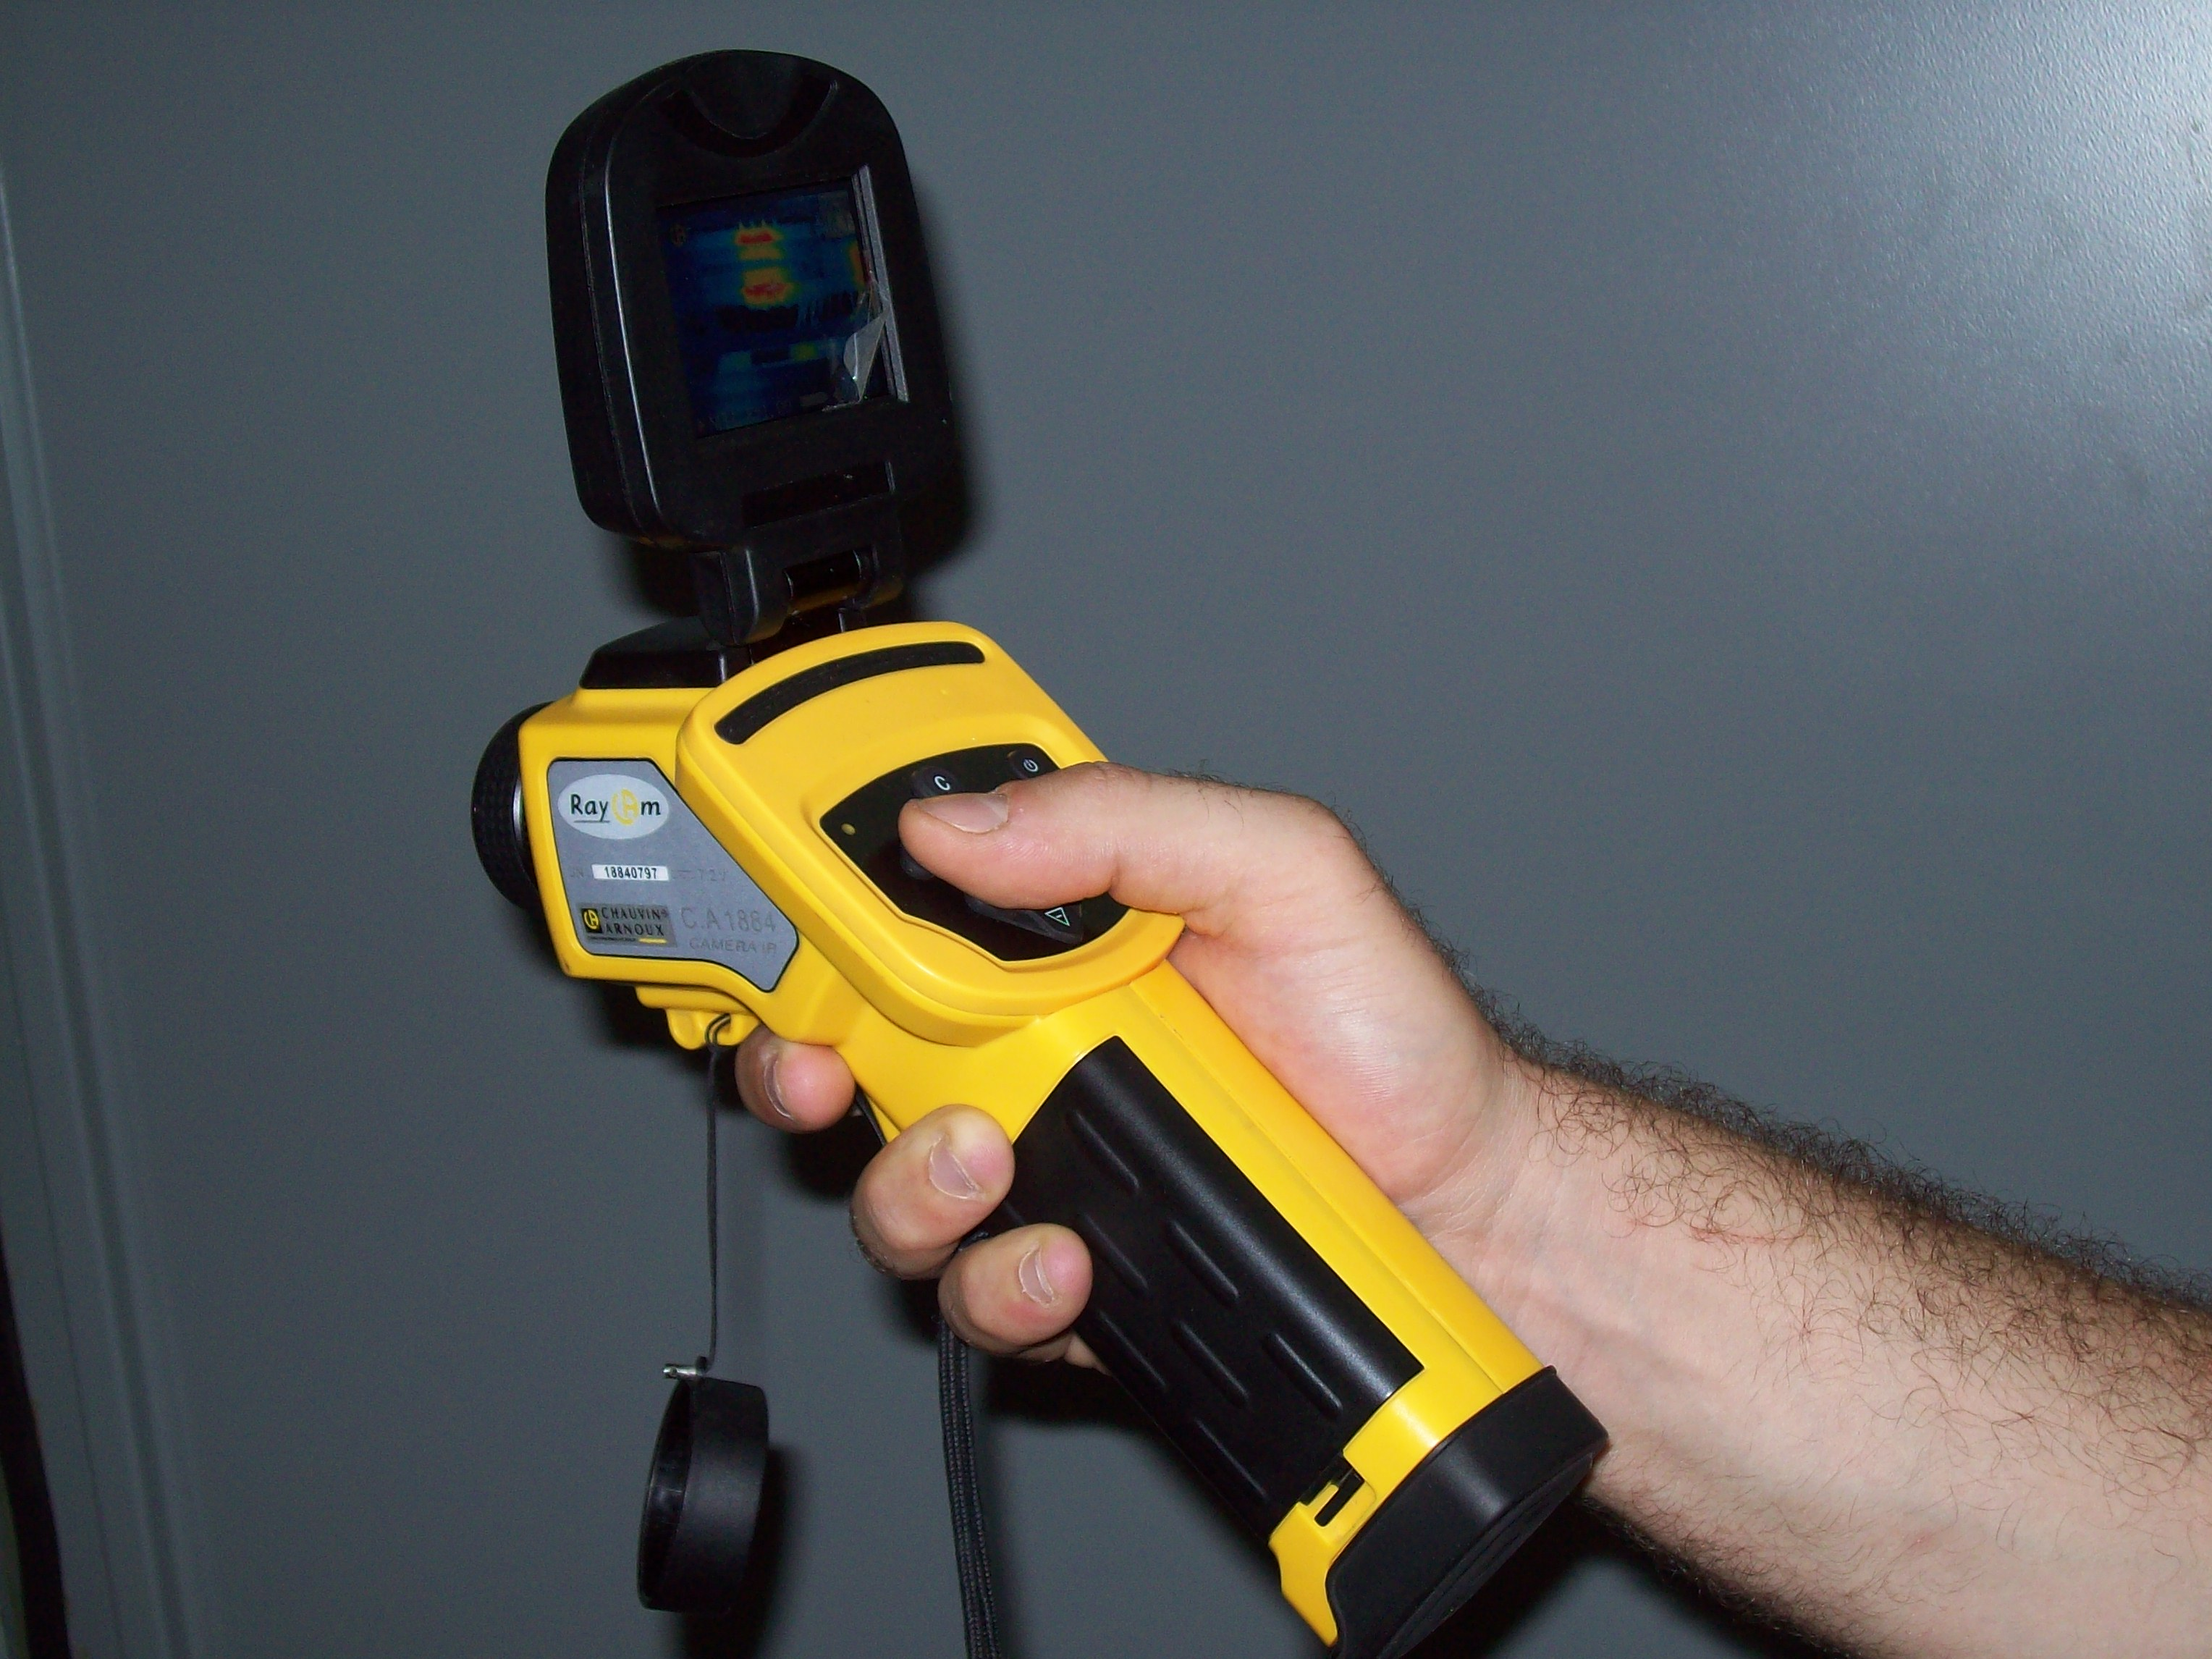
\includegraphics[scale=0.07]{./Figures/infra.JPG}
\caption{Caméra thermographique infrarouge}
\end{figure}
Celle ci est caractérisée par :

\begin{itemize}
\item Sa plage de mesure de température.
\item Sa précision
\item Sa bande spectrale.
\item Sa résolution optique
\item Son champ de visée instantanée%dafuq
\item Son logiciel d'exploitation.

\end{itemize}
Il est  aussi  nécessaire de se procurer de :  
 
 \begin{itemize}
 
\item Un appareil photo
\item Une pince ampère-métrique
\item Un ordinateur équipé d'un logiciel d'exploitation spécifique. \end{itemize}
\subsubsection{La pratique}
Une fois arrivé sur le lieu de mesure, on met en marche la caméra thermique. 

Pour faire une analyse, on prend toujours deux points de mesures : Un qui est visiblement en défaut et un autre qui n'en est pas. Ceci dans le but de mesurer une différence de température et en tirer des conclusions.       

On prend aussi une photo de l'appareil en question pour le repérer dans l'armoire électrique et le situer exactement (voir figure \ref{fig:analyse_thermo}).

\begin{figure}[ht]
\centering
\subfigure[Image infrarouge]{
	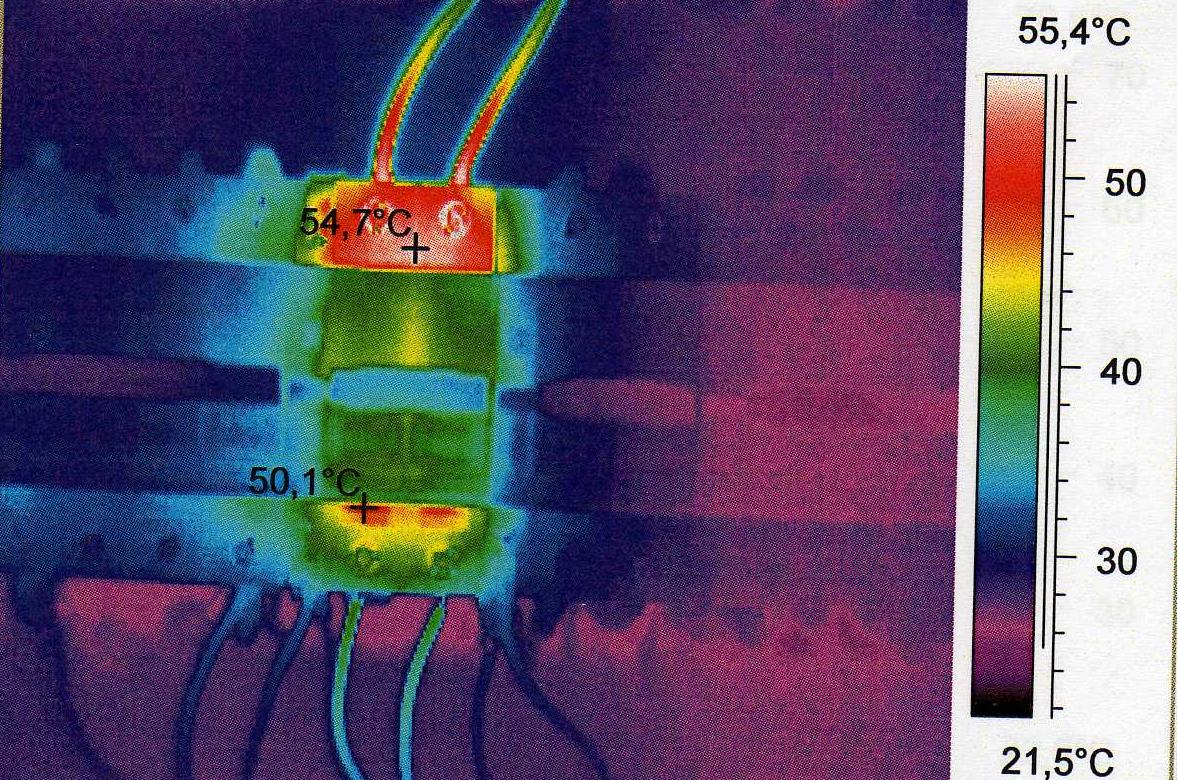
\includegraphics[scale=0.26]{./Figures/vue_infra.jpg}
		\label{fig:vue_infra}

}
\subfigure[Image réelle]{
	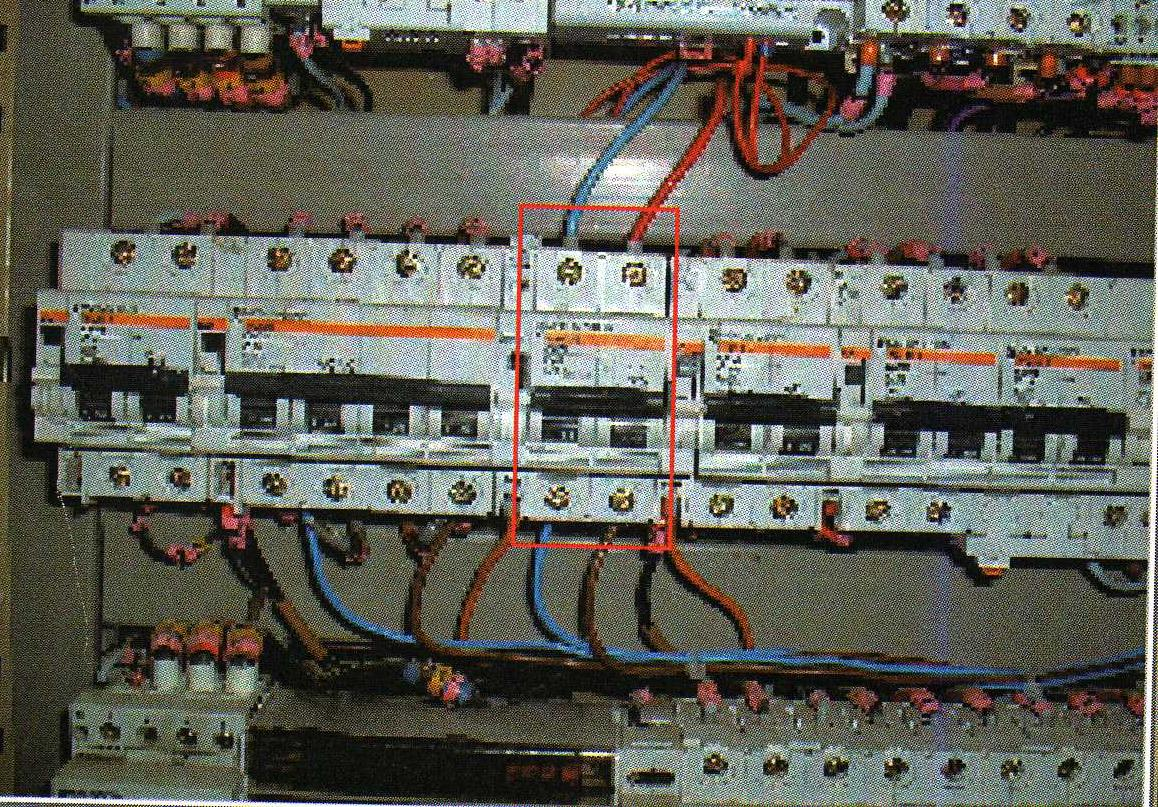
\includegraphics[scale=0.29,trim=6cm 0cm 4cm 2cm,clip=true]{./Figures/vue_normal.jpg}

	\label{fig:vue_reelle}
}
\caption{Analyse thermographique}
\label{fig:analyse_thermo}
\end{figure}
\pagebreak
\paragraph{Commentaires}
On voit bien  que toute la zone d'arrivée du courant est rouge. Cela signifie qu'il y a un échauffement important. La seule cause plausible est que l'appareil n'est pas conçu pour recevoir  une si grand intensité. Dans ce cas, il faut remplacer l'appareil par un autre de calibre supérieur.
\subsubsection{Conclusion}
L'analyse thermographique peut nous aider à anticiper et prévenir la coupure ou l'arrêt intempestif et surtout éviter les incendies d'origine électrique.

Elle se fait sous tension et donc, elle nous évite les pertes de production.

Cependant elle présente un inconvénient majeur à savoir le temps. En effet, la durée passée pour faire le tour de tous les appareils électriques est important. Seule une bonne organisation peut pallier ce problème.%voir verbe

Le prix  élevé de la caméra infrarouge peut être considéré comme un autre inconvénient. Néanmoins, vu les problèmes qu'elle peut nous éviter, on reste dans une politique gagnante.


\subsection{Analyse d'énergie}
\subsubsection{Principe et But}
L'analyse d'énergie est l'un des paramètres nécessaires  de la maintenance  préventive. 

Elle permet :

\begin{itemize}
\item La mesure des paramètres de tension, courant et puissances utiles jusqu'au diagnostic complet d'une installation électrique

\item Capture et enregistrement simultané de tous les paramètres transitoires,  alarmes et formes d'ondes
\end{itemize}

Cette technique est principalement appliquée sur les moteurs électriques en état de fonctionnement.
Elle sert à identifier les surcharges et les déséquilibres de courants.

\subsubsection{Matériel de l'analyse}


\textbf{L'analyseur C.A 8334 : }
Cet analyseur d'énergie électrique permet d'obtenir non seulement une image instantanée du réseau en question mais aussi le suivie leurs variation dans le temps.

\begin{figure}[hbtp]
\centering
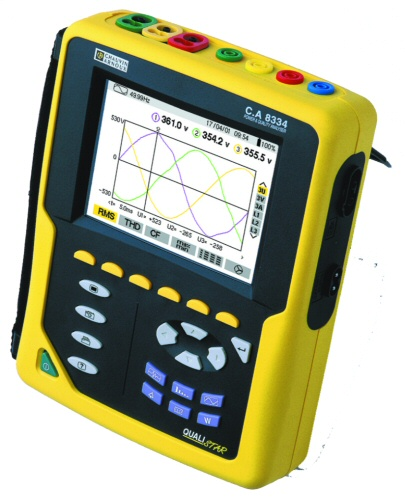
\includegraphics[scale=1.5]{./Figures/analyseur_energie.jpg}
\caption{Analyseur C.A 8334}
\end{figure}



Les mesures prises peuvent être directement visualisées  sur l'appareil. Pour une traitement plus profond, l'utilisateur peut récupérer ces données dans son ordinateur grâce au logiciel d'exploitation intégré.
\begin{figure}[hbtp]
\centering
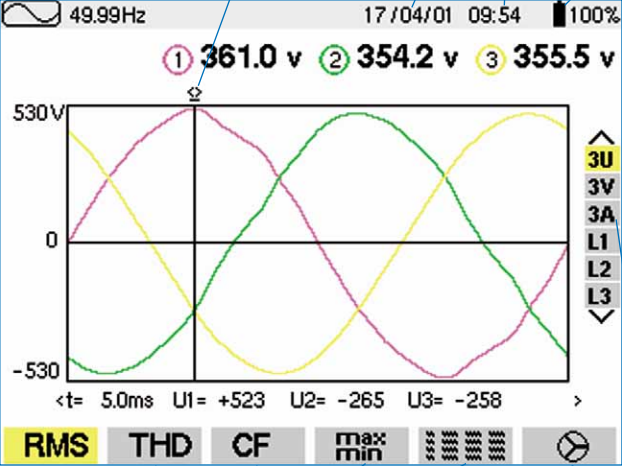
\includegraphics[scale=0.5]{./Figures/Ecran_analyseur.png}
\caption{Affichage analyseur d'énergie}
\end{figure}
\subsubsection{La pratique}

Étant donnée que l'analyse d'énergie se déroule lors du fonctionnement du moteur, elle  présente un risque important pour l'utilisateur et le réseau.

Plusieurs mesures de sécurité\footnote{Pour plus de détails consulter l'annexe \uppercase\expandafter{\romannumeral 6}} sont appliquées :

\begin{itemize}
\item Consignation du tiroir 
\item Port d'un casque spécial (protection de l'arc électrique)
\item Port des gants isolants

\end{itemize}

On branche les six câbles de mesure (trois pour la mesure des courants et trois pour les voltages). 

La mesure prend environ dix-minutes. On peut suivre l'évolution des caractéristiques sur l'écran de l'appareil. On constate que les premiers chiffres sont dans les normes.

On débranche l'appareil du réseau et on le relie à un ordinateur pour obtenir un rapport plus détaillé.

L'analyse  des données collectées seule ne suffit pas à émettre un verdict. Il est alors nécessaire  de se référer à l'historique accessible à partir du GMAO\footnote{Se référer à l'annexe \uppercase\expandafter{\romannumeral 5} } pour observer l'évolution. 

Pour le cas d'un cas moteur (comme c'est le cas ici), on vérifie le déséquilibre des phases. On trouve une valeur dans les normes.
 
\subsubsection{Conclusion}
L'analyse d'énergie est une technique très utilisée dans la maintenance des réseaux électriques. Sa puissance relève des fonctionnalités de  l'analyseur employé et de son logiciel de traitement. Ceci  pose en général un léger compromis au niveau financier. %compromis

\subsection{Remplacement du relai MiCOM P120}
\subsubsection{Situation du problème}
Les relais de surintensité de la gamme  MiCOM P120  sont les relais à maximum de courant universels d'ALSTOM. Les relais de la gamme MiCOM P120 sont conçus pour contrôler, protéger et superviser tant les installations industrielles que les réseaux de distribution publique, les postes sources.

Dans la centrale, ces relais sont utilisés pour la  protection des surintensités dans le neutre d'un transformateur.

Normalement, des tests d'intervalles réguliers sont planifiés pour assurer le bon fonctionnement et la disponibilité du relai. Cependant, les pannes arrivent et on est passé d'une maintenance préventive en une maintenance corrective.
\pagebreak
\subsubsection{Matériel}
Le test d'un relai peut se faire dans deux situations :

\begin{itemize}
\item Un test de routine lors de la prévention préventive
\item Une vérification d'un nouveau relai
\end{itemize}
Dans les deux cas, il faut mettre le relai dans son   environnement de travail.
Pour cela, les techniciens ont recourt à la valise d'injection.
Cette dernière  peut être paramétrée pour simuler les conditions de fonctionnement du relais. 

\begin{figure}[hbtp]
\centering
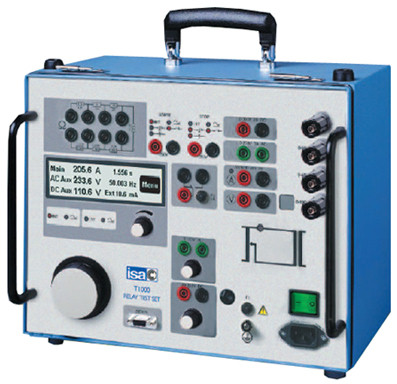
\includegraphics[scale=0.4]{./Figures/T1000.jpg}
\caption{Valise d'injection T1000 - Relay Test Set}
\end{figure}


\subsubsection{La pratique}
La démarche à suivre est simple mais présente un risque de déclenchement de la turbine à vapeur. Elle peut être résumée dans les étapes suivantes :

\begin{itemize}
\item Déconnexion des deux contacts de la chaine de trip du relai
\item Démontage de l'ancien relai et fixation du nouveau testé et configuré au préalable
\item Vérification du bon fonctionnement du nouveau relais, vérification de la valeur du courant mesurée et vérification des deux contacts de trip (les deux contacts doivent être ouvert)
\item Connexion de nouveau des deux contacts de trip
\item Vérification  finale du bon fonctionnement du relais et d'absence d'alarme au DCS
\end{itemize}
\subsection{Vérification des batteries du Groupe Diesel}
\subsubsection{Situation du problème}
Outre son besoin en combustible, la turbine à gaz nécessite une constante lubrification pour éviter le frottement des pièces mécaniques. Cette opération ne  doit en aucun cas être suspendue. C'est pourquoi, en cas de problème l'alimentation des pompes de graissage est maintenue en premier lieu  par des batteries de secours et en deuxième lieu à travers les Groupes Diesel. Ces groupes sont des mini-turbines fonctionnant avec le Diesel et sont lancés par un moteur consommant un courant continu. 

Le but de cette activité est d'effectuer quelques testes afin d'assurer la disponibilité continue des batteries du Groupe Diesel.
\subsubsection{Matériel}
Dans le suivi de l'état des batteries, on s'intéresse au voltage et à la densité de l'acide.
Pour la mesure de voltage on utilise un multimètre.
Quant à la densité, elle est mise en évidence par un densimètre. Il s'agit tout simplement d'un flotteur dont le volume immergé dépend de la densité  du liquide dans lequel il et plongé. 
Son principe de fonctionnement est donc lié à la poussée d'Archimède. 
\begin{figure}[h]

  \begin{minipage}[ht]{7cm}
        \centering
	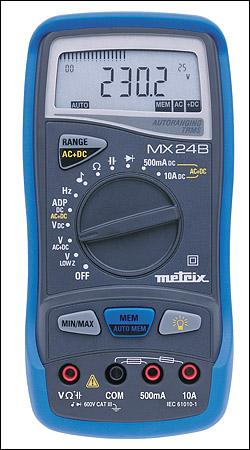
\includegraphics[scale=0.4]{./Figures/multimetre.jpg}
		\label{fig:Multimere}
		\caption{Multimètre}
    \end{minipage}
    \begin{minipage}[ht]{8cm}
        \centering
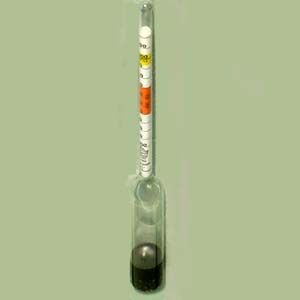
\includegraphics[scale=01]{./Figures/densimetre.jpg}

	\label{fig:Densimetre}
			\caption{Densimètre}

    \end{minipage}
\end{figure}

\subsubsection{La pratique}
Équipé de notre matériel, on se dirige vers l'emplacement des Groupes Diesel.
On ouvre le disjoncteur principale et on commence notre tâche.
Dans un premier temps on enlève l'acide accumulé sur les cosses et on mesure le voltage. La valeur trouvée doit être dans les environs des 13 V.

Dans un deuxième temps, on ouvre les bouchons et on vérifie le niveau d'acide. Si le niveau est trop bas, on le complète avec l'eau distillée. On finit par noter la densité de l'acide qui nous renseigne sur la concentration. La valeur de la densité doit être dans les alentours de 1.26. Si cette dernière est faible, on doit ajouter de l'acide. 
